\documentclass{standalone}
\usepackage{tikz}
\usetikzlibrary{patterns, positioning}
\usepackage[sfdefault]{ClearSans} %% option 'sfdefault' activates Clear Sans as the default text font
\usepackage[T1]{fontenc}

\begin{document}
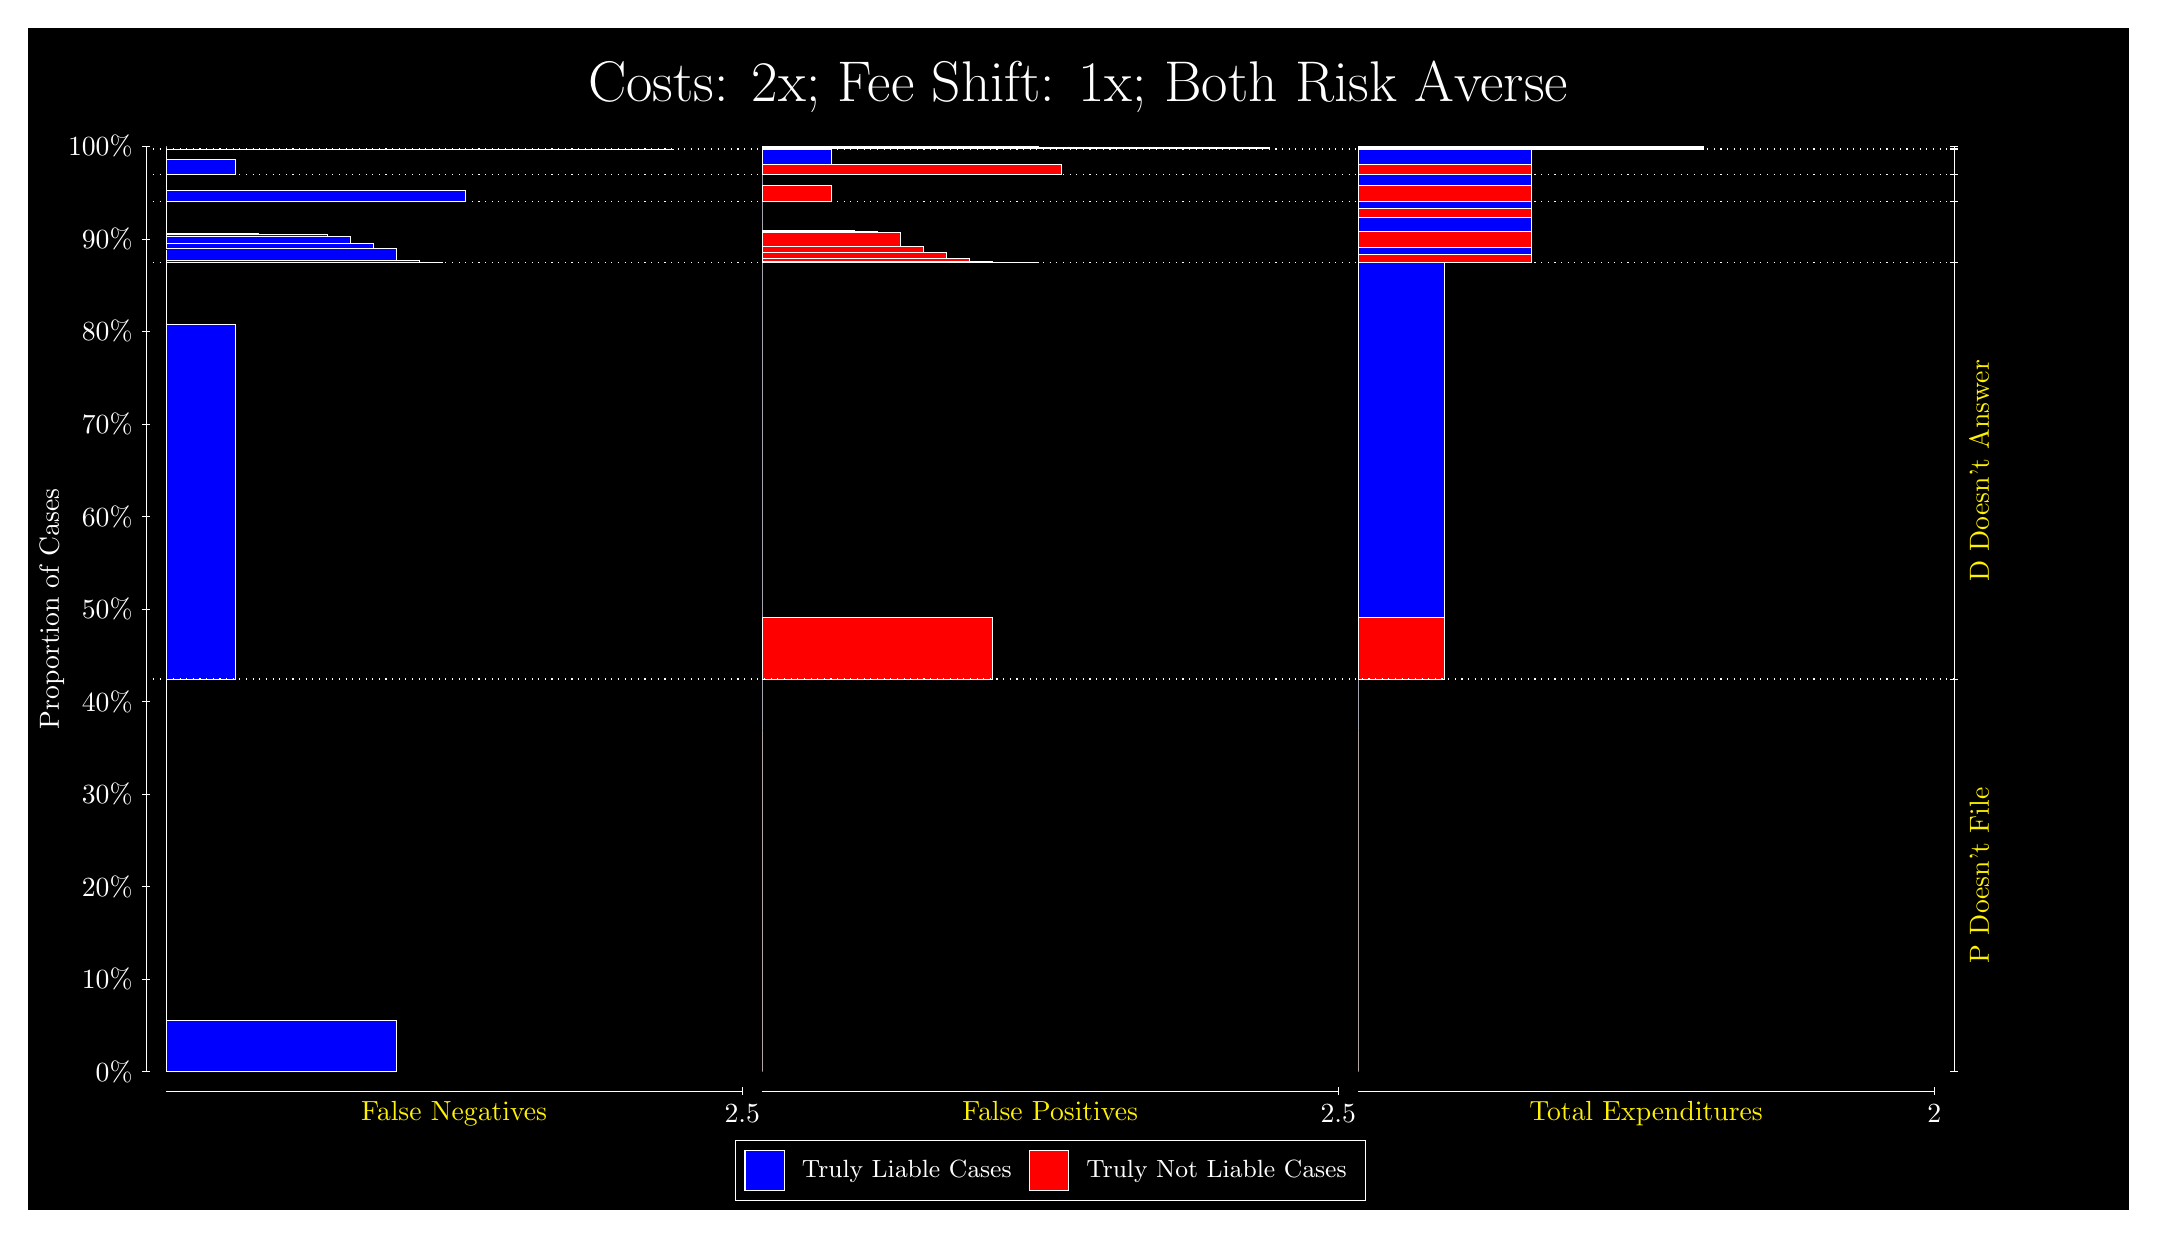
\begin{tikzpicture}
\draw[fill=black] (0,0) rectangle (26.667,15);
\draw[text=white] (0,13.5) rectangle (26.667,15) node[midway] {\huge Costs: 2x; Fee Shift: 1x; Both Risk Averse};
\draw[white, very thin] (1.5,1.75) -- (1.5,13.5);
\node[rotate=90, text=white, anchor=center] at (0.3, 7.625) {Proportion of Cases};
\draw[white, very thin] (1.45,1.75) -- (1.55,1.75);
\node[text=white, anchor=east] at (1.45, 1.75) {0\%};
\draw[white, very thin] (1.45,2.925) -- (1.55,2.925);
\node[text=white, anchor=east] at (1.45, 2.925) {10\%};
\draw[white, very thin] (1.45,4.1) -- (1.55,4.1);
\node[text=white, anchor=east] at (1.45, 4.1) {20\%};
\draw[white, very thin] (1.45,5.275) -- (1.55,5.275);
\node[text=white, anchor=east] at (1.45, 5.275) {30\%};
\draw[white, very thin] (1.45,6.45) -- (1.55,6.45);
\node[text=white, anchor=east] at (1.45, 6.45) {40\%};
\draw[white, very thin] (1.45,7.625) -- (1.55,7.625);
\node[text=white, anchor=east] at (1.45, 7.625) {50\%};
\draw[white, very thin] (1.45,8.8) -- (1.55,8.8);
\node[text=white, anchor=east] at (1.45, 8.8) {60\%};
\draw[white, very thin] (1.45,9.975) -- (1.55,9.975);
\node[text=white, anchor=east] at (1.45, 9.975) {70\%};
\draw[white, very thin] (1.45,11.15) -- (1.55,11.15);
\node[text=white, anchor=east] at (1.45, 11.15) {80\%};
\draw[white, very thin] (1.45,12.325) -- (1.55,12.325);
\node[text=white, anchor=east] at (1.45, 12.325) {90\%};
\draw[white, very thin] (1.45,13.5) -- (1.55,13.5);
\node[text=white, anchor=east] at (1.45, 13.5) {100\%};

\draw[white, very thin] (24.457,1.75) -- (24.457,13.5);
\draw[white, very thin] (24.407,1.75) -- (24.507,1.75);
\node[anchor=west] at (24.407, 1.75) {};
\draw[white, very thin] (24.407,6.7349) -- (24.507,6.7349);
\node[anchor=west] at (24.407, 6.7349) {};
\draw[white, very thin] (24.407,12.024) -- (24.507,12.024);
\node[anchor=west] at (24.407, 12.024) {};
\draw[white, very thin] (24.407,12.802) -- (24.507,12.802);
\node[anchor=west] at (24.407, 12.802) {};
\draw[white, very thin] (24.407,13.143) -- (24.507,13.143);
\node[anchor=west] at (24.407, 13.143) {};
\draw[white, very thin] (24.407,13.46) -- (24.507,13.46);
\node[anchor=west] at (24.407, 13.46) {};
\draw[white, very thin] (24.407,13.478) -- (24.507,13.478);
\node[anchor=west] at (24.407, 13.478) {};
\draw[white, very thin] (24.407,13.5) -- (24.507,13.5);
\node[anchor=west] at (24.407, 13.5) {};

\draw[white, very thin, fill=blue] (1.75,1.75) rectangle (4.6775,2.4018);
\draw[white, very thin, fill=red] (1.75,2.4018) rectangle (1.75,6.7349);
\draw[white, very thin, fill=blue] (1.75,6.7349) rectangle (2.6283,11.244);
\draw[white, very thin, fill=red] (1.75,11.244) rectangle (1.75,12.024);
\draw[white, very thin, fill=blue] (1.75,12.024) rectangle (5.2631,12.031);
\draw[white, very thin, fill=blue] (1.75,12.031) rectangle (4.9703,12.055);
\draw[white, very thin, fill=blue] (1.75,12.055) rectangle (4.6775,12.199);
\draw[white, very thin, fill=blue] (1.75,12.199) rectangle (4.3848,12.2);
\draw[white, very thin, fill=blue] (1.75,12.2) rectangle (4.3848,12.274);
\draw[white, very thin, fill=blue] (1.75,12.274) rectangle (4.092,12.359);
\draw[white, very thin, fill=blue] (1.75,12.359) rectangle (3.7993,12.378);
\draw[white, very thin, fill=blue] (1.75,12.378) rectangle (3.5065,12.387);
\draw[white, very thin, fill=blue] (1.75,12.387) rectangle (3.2138,12.388);
\draw[white, very thin, fill=blue] (1.75,12.388) rectangle (2.921,12.391);
\draw[white, very thin, fill=red] (1.75,12.391) rectangle (1.75,12.802);
\draw[white, very thin, fill=blue] (1.75,12.802) rectangle (5.5558,12.94);
\draw[white, very thin, fill=red] (1.75,12.94) rectangle (1.75,13.143);
\draw[white, very thin, fill=blue] (1.75,13.143) rectangle (2.6283,13.33);
\draw[white, very thin, fill=red] (1.75,13.33) rectangle (1.75,13.46);
\draw[white, very thin, fill=blue] (1.75,13.46) rectangle (8.1906,13.467);
\draw[white, very thin, fill=red] (1.75,13.467) rectangle (1.75,13.478);
\draw[white, very thin, fill=red] (1.75,13.478) rectangle (1.75,13.484);
\draw[white, very thin, fill=blue] (1.75,13.484) rectangle (1.75,13.5);
\draw[white, very thin, fill=red] (9.3189,1.75) rectangle (9.3189,6.083);
\draw[white, very thin, fill=blue] (9.3189,6.083) rectangle (9.3189,6.7349);
\draw[white, very thin, fill=red] (9.3189,6.7349) rectangle (12.246,7.5151);
\draw[white, very thin, fill=blue] (9.3189,7.5151) rectangle (9.3189,12.024);
\draw[white, very thin, fill=red] (9.3189,12.024) rectangle (12.832,12.026);
\draw[white, very thin, fill=red] (9.3189,12.026) rectangle (12.539,12.027);
\draw[white, very thin, fill=red] (9.3189,12.027) rectangle (12.246,12.041);
\draw[white, very thin, fill=red] (9.3189,12.041) rectangle (11.954,12.072);
\draw[white, very thin, fill=red] (9.3189,12.072) rectangle (11.661,12.157);
\draw[white, very thin, fill=red] (9.3189,12.157) rectangle (11.368,12.235);
\draw[white, very thin, fill=red] (9.3189,12.235) rectangle (11.075,12.403);
\draw[white, very thin, fill=red] (9.3189,12.403) rectangle (10.783,12.425);
\draw[white, very thin, fill=red] (9.3189,12.425) rectangle (10.49,12.435);
\draw[white, very thin, fill=blue] (9.3189,12.435) rectangle (9.9044,12.438);
\draw[white, very thin, fill=blue] (9.3189,12.438) rectangle (9.6116,12.439);
\draw[white, very thin, fill=blue] (9.3189,12.439) rectangle (9.3189,12.802);
\draw[white, very thin, fill=red] (9.3189,12.802) rectangle (10.197,13.005);
\draw[white, very thin, fill=blue] (9.3189,13.005) rectangle (9.3189,13.143);
\draw[white, very thin, fill=red] (9.3189,13.143) rectangle (13.125,13.274);
\draw[white, very thin, fill=blue] (9.3189,13.274) rectangle (10.197,13.46);
\draw[white, very thin, fill=red] (9.3189,13.46) rectangle (9.3189,13.471);
\draw[white, very thin, fill=blue] (9.3189,13.471) rectangle (9.3189,13.478);
\draw[white, very thin, fill=red] (9.3189,13.478) rectangle (15.759,13.484);
\draw[white, very thin, fill=blue] (9.3189,13.484) rectangle (12.832,13.5);
\draw[white, very thin, fill=red] (16.888,1.75) rectangle (16.888,6.083);
\draw[white, very thin, fill=blue] (16.888,6.083) rectangle (16.888,6.7349);
\draw[white, very thin, fill=red] (16.888,6.7349) rectangle (17.986,7.5151);
\draw[white, very thin, fill=blue] (16.888,7.5151) rectangle (17.986,12.024);
\draw[white, very thin, fill=red] (16.888,12.024) rectangle (19.083,12.125);
\draw[white, very thin, fill=blue] (16.888,12.125) rectangle (19.083,12.221);
\draw[white, very thin, fill=red] (16.888,12.221) rectangle (19.083,12.423);
\draw[white, very thin, fill=blue] (16.888,12.423) rectangle (19.083,12.599);
\draw[white, very thin, fill=red] (16.888,12.599) rectangle (19.083,12.707);
\draw[white, very thin, fill=blue] (16.888,12.707) rectangle (19.083,12.802);
\draw[white, very thin, fill=red] (16.888,12.802) rectangle (19.083,13.005);
\draw[white, very thin, fill=blue] (16.888,13.005) rectangle (19.083,13.143);
\draw[white, very thin, fill=red] (16.888,13.143) rectangle (19.083,13.274);
\draw[white, very thin, fill=blue] (16.888,13.274) rectangle (19.083,13.46);
\draw[white, very thin, fill=red] (16.888,13.46) rectangle (21.279,13.471);
\draw[white, very thin, fill=blue] (16.888,13.471) rectangle (21.279,13.478);
\draw[white, very thin, fill=red] (16.888,13.478) rectangle (21.279,13.484);
\draw[white, very thin, fill=blue] (16.888,13.484) rectangle (21.279,13.5);
\draw[white, dotted] (1.5,6.7349) -- (24.457,6.7349);
\draw[white, dotted] (1.5,12.024) -- (24.457,12.024);
\draw[white, dotted] (1.5,12.802) -- (24.457,12.802);
\draw[white, dotted] (1.5,13.143) -- (24.457,13.143);
\draw[white, dotted] (1.5,13.46) -- (24.457,13.46);
\draw[white, dotted] (1.5,13.478) -- (24.457,13.478);
\draw[white, very thin] (1.75,1.5) -- (9.0689,1.5);
\node[text=yellow, anchor=north] at (5.4094, 1.5) {False Negatives};
\draw[white, very thin] (9.0689,1.45) -- (9.0689,1.55);
\node[text=white, anchor=north] at (9.0689, 1.45) {2.5};

\draw[white, very thin] (9.3189,1.5) -- (16.638,1.5);
\node[text=yellow, anchor=north] at (12.978, 1.5) {False Positives};
\draw[white, very thin] (16.638,1.45) -- (16.638,1.55);
\node[text=white, anchor=north] at (16.638, 1.45) {2.5};

\draw[white, very thin] (16.888,1.5) -- (24.207,1.5);
\node[text=yellow, anchor=north] at (20.547, 1.5) {Total Expenditures};
\draw[white, very thin] (24.207,1.45) -- (24.207,1.55);
\node[text=white, anchor=north] at (24.207, 1.45) {2};

\node[text=yellow, centered, rotate=90] at (24.777, 4.2424) {P Doesn't File};
\node[text=yellow, centered, rotate=90] at (24.777, 9.3796) {D Doesn't Answer};






\draw (12.978300999999998,1.5) node[draw=none] (baseCoordinate) {};
\begin{scope}[align=center]
        \matrix[scale=0.5, draw=white, below=0.5cm of baseCoordinate, nodes={draw}, column sep=0.1cm]{
            \node[rectangle, draw, minimum width=0.5cm, minimum height=0.5cm, fill=blue] {}; &
            \node[draw=none, font=\small, text=white] (B) {Truly Liable Cases}; &
            \node[rectangle, draw, minimum width=0.5cm, minimum height=0.5cm, fill=red] {}; &
            \node[draw=none, font=\small, text=white] (B) {Truly Not Liable Cases}; \\
            };
\end{scope}

\end{tikzpicture}
\end{document}